\section{随机梯度方法}
\label{sec:opt-sto-sgd}

上一节固定了目标，并看到单项读数可能指向上坡。本节把这样的读数直接代入梯度下降，研究“单步可能变坏、平均仍在变好”这件事怎样精确表述。工具是条件期望：给定到目前为止发生的一切，下一步读数的平均是什么。由此得到一条单步递推，后面的常数步长误差、递减步长速率和返回点的选择都从它推出。

\subsection{条件无偏与读数误差}
\label{sec:opt-sto-unbiased}

\paragraph{历史与条件期望}
随机算法的第$t$步发生之前，初值$\bm x^{(0)}$以及前$t$步抽到的下标$i^{(0)},\dots,i^{(t-1)}$都已经确定，迭代点$\bm x^{(t)}$是它们的函数。把这些已经观察到的随机量所含的信息记为\emph{历史}$\mathcal F^{(t)}$，严格地说，它是由这些随机量生成的$\sigma$代数。给定历史后的条件期望记作
\[
  \mathbb E_t[\,\cdot\,]=\mathbb E\bigl[\,\cdot\mid\mathcal F^{(t)}\bigr].
\]
本章只用条件期望的三条基本性质：由历史决定的量（如$\bm x^{(t)}$、$\nabla f(\bm x^{(t)})$）可以像常数一样提到$\mathbb E_t$外面；若新的下标$i^{(t)}$与历史独立，则$\mathbb E_t[\phi(\bm x^{(t)},i^{(t)})]$等于把$\bm x^{(t)}$当作固定点、只对$i^{(t)}$求平均；以及全期望公式$\mathbb E[\mathbb E_t[Z]]=\mathbb E[Z]$。这些性质的严格陈述和证明见\BookChapterRef{chap:conditional-expectation}{卷二“条件期望与条件分布”章}。

\paragraph{条件无偏的读数}
第$t$步算法得到一个向量$\bm g^{(t)}$，用来代替$\nabla f(\bm x^{(t)})$。我们需要的不是“平均来说$\bm g^{(t)}$与梯度差不多”，而是“站在当前点、看着已有的历史，下一次读数的平均正好是这里的梯度”。

\begin{definition}[条件无偏读数]
\label{def:opt-sto-unbiased}
设$\bm g^{(t)}$是可积随机向量。若
\[
  \mathbb E_t\bigl[\bm g^{(t)}\bigr]=\nabla f(\bm x^{(t)})
\]
几乎必然成立，称$\bm g^{(t)}$是$\nabla f$在$\bm x^{(t)}$处的\term{条件无偏}（conditionally unbiased）读数，也称\term{随机梯度}（stochastic gradient）。
\end{definition}

对有限和~\eqref{eq:opt-sto-finite-sum}，若$i^{(t)}$在$\{1,\dots,n\}$上均匀分布且与历史独立，则$\bm g^{(t)}=\nabla f_{i^{(t)}}(\bm x^{(t)})$满足$\mathbb E_t[\bm g^{(t)}]=\frac1n\sum_i\nabla f_i(\bm x^{(t)})=\nabla f(\bm x^{(t)})$，这正是上述第二条性质。条件版本比无条件的$\mathbb E[\bm g^{(t)}]=\mathbb E[\nabla f(\bm x^{(t)})]$强得多：如果抽样规则看了当前位置，例如在三点例中$x>2$时总抽第一项、$x<2$时总抽第三项，那么每一步的读数都系统性地偏离当地梯度，即使把所有时刻混在一起平均，偏差也可能互相抵消而看不出来。后面的单步分析在每个固定历史下取平均，所以需要的正是条件无偏。

\paragraph{读数的分解}
一般的读数未必无偏，例如被截断、量化或者用了过时的参数。把它拆成三部分：
\begin{equation}
\label{eq:opt-sto-reading-split}
\begin{aligned}
  \bm g^{(t)}&=\nabla f(\bm x^{(t)})+\bm\beta^{(t)}+\bm\xi^{(t)},\\
  \bm\beta^{(t)}&=\mathbb E_t[\bm g^{(t)}]-\nabla f(\bm x^{(t)}),\qquad
  \bm\xi^{(t)}=\bm g^{(t)}-\mathbb E_t[\bm g^{(t)}].
\end{aligned}
\end{equation}
$\bm\beta^{(t)}$是\emph{条件偏差}，由历史决定；$\bm\xi^{(t)}$是\emph{噪声}，满足$\mathbb E_t[\bm\xi^{(t)}]=\bm0$。两者需要分别控制，常用的假设是$\lVert\bm\beta^{(t)}\rVert_2\leq B$与$\mathbb E_t\lVert\bm\xi^{(t)}\rVert_2^2\leq\sigma^2$。条件无偏就是$\bm\beta^{(t)}=\bm0$。此时把$\lVert\bm g^{(t)}\rVert_2^2$展开，交叉项$2\langle\nabla f(\bm x^{(t)}),\bm\xi^{(t)}\rangle$的条件期望为零，得到后面反复使用的恒等式
\begin{equation}
\label{eq:opt-sto-second-moment}
  \mathbb E_t\lVert\bm g^{(t)}\rVert_2^2=\lVert\nabla f(\bm x^{(t)})\rVert_2^2+\mathbb E_t\lVert\bm\xi^{(t)}\rVert_2^2 .
\end{equation}
读数的平均平方长度等于真梯度的平方长度加上噪声的方差：噪声只会让读数变长，不会让它变短。

\paragraph{无偏不等于下降，也不等于方差小}
在三点例的$x=3$处，三个读数$3,2,-2$以等概率出现，平均为$1$。读数$-2$与真梯度方向相反，沿它走一步会上坡，这种情况的概率是$1/3$。噪声的方差为$\mathbb E_t(\xi^{(t)})^2=\frac13\bigl(2^2+1^2+3^2\bigr)=\frac{14}3$，远大于真梯度的平方$1$。由于每一项曲率相同，噪声$\xi^{(t)}=(x-c_{i^{(t)}})-(x-2)=2-c_{i^{(t)}}$与$x$无关，这个方差在任何点都是$14/3$；即使站在最小点$x^\star=2$，读数仍是$2,1,-3$之一，算法仍会被推离最小点。图~\ref{fig:opt-sto-gradient-fan}在二维最小二乘上画出同样的现象：十个逐项下降方向散成一把扇子，其中三个与平均方向成钝角，只有平均才指向等高线的内侧。

\begin{figure}[!htbp]
  \centering
  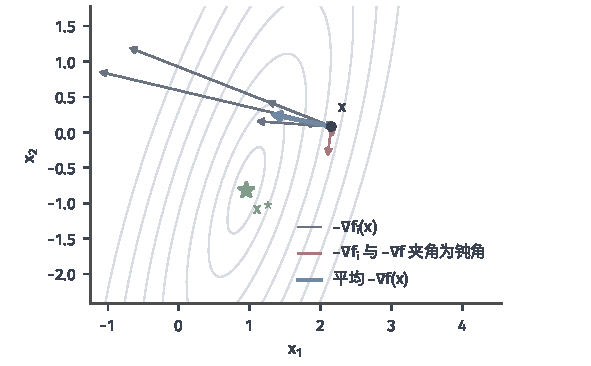
\includegraphics[width=100mm]{figures/03-optimization-evolution-and-signals/01-optimization/matplotlib/c6-gradient-fan/figure.pdf}
  \caption{一点处的逐项读数。目标是$n=10$、$d=2$的岭回归最小二乘，灰色曲线为等高线，星号为最小点。从黑点$\bm x$出发的细箭头是逐项下降方向$-\nabla f_i(\bm x)$（按$0.35$倍画出），其中红色的三个与平均方向夹角为钝角，单独沿它们走一小步会使目标上升；粗蓝箭头是它们的平均$-\nabla f(\bm x)$。数据由固定种子生成，参数见图源记录。}
  \label{fig:opt-sto-gradient-fan}
\end{figure}

\subsection{随机梯度下降与步长}
\label{sec:opt-sto-sgd-step}

\paragraph{一轮更新}
把读数代入梯度下降，就得到\term{随机梯度下降}（stochastic gradient descent）。下面的算法写清每一轮的四个动作：抽样、读取、更新和记录。步长$\eta^{(t)}$必须在抽取$i^{(t)}$之前确定，即由历史决定；否则步长与读数相关，条件期望就不能把它们分开处理。

\begin{algorithm}[随机梯度下降]
\label{alg:opt-sto-sgd}
\begin{algorithmic}[1]
\Require 初值$\bm x^{(0)}$，步长序列$\eta^{(0)},\eta^{(1)},\dots$（由历史决定），轮数$T$，抽样分布
\Ensure 返回点（最后一点、加权平均点或随机选出的迭代点，见第~\ref{sec:opt-sto-return}节）
\For{$t=0,1,\dots,T-1$}
  \State 与历史独立地抽取下标$i^{(t)}$
  \State 读取$\bm g^{(t)}=\nabla f_{i^{(t)}}(\bm x^{(t)})$
  \State $\bm x^{(t+1)}=\bm x^{(t)}-\eta^{(t)}\bm g^{(t)}$
  \State 按所选返回规则更新记录（如累加$\eta^{(t)}\bm x^{(t)}$）
\EndFor
\end{algorithmic}
\end{algorithm}

每轮读取一项，计算$O(d)$，额外存储只有返回规则所需的一个向量。每轮\emph{重新}抽样是关键。若始终使用同一个下标$i$，算法就是对$f_i$的普通梯度下降，收敛到$f_i$的最小点而不是$f$的最小点：在三点例中始终读第三项，迭代会走向$5$。重新抽样让不同项的偏向在多步中相互抵消。

\paragraph{代入光滑上界}
随机梯度的单步分析与梯度下降相同，只是在最后对新下标取条件期望。设$f$是$L$光滑的，第~\ref{chap:opt-smooth}章的下降引理给出$f(\bm x+\bm p)\leq f(\bm x)+\langle\nabla f(\bm x),\bm p\rangle+\tfrac L2\lVert\bm p\rVert_2^2$。

\begin{lemma}[随机梯度的单步下降]
\label{lem:opt-sto-one-step}
设$f$在$\mathbb R^d$上$L$光滑，$\bm g^{(t)}$条件无偏且$\mathbb E_t\lVert\bm g^{(t)}-\nabla f(\bm x^{(t)})\rVert_2^2\leq\sigma^2$，步长$\eta=\eta^{(t)}$由历史决定。则$\bm x^{(t+1)}=\bm x^{(t)}-\eta\bm g^{(t)}$满足
\begin{equation}
\label{eq:opt-sto-one-step}
  \mathbb E_t f(\bm x^{(t+1)})\leq f(\bm x^{(t)})-\eta\Bigl(1-\frac{L\eta}2\Bigr)\lVert\nabla f(\bm x^{(t)})\rVert_2^2+\frac{L\eta^2}{2}\sigma^2 .
\end{equation}
\end{lemma}

\begin{proof}
取$\bm p=-\eta\bm g^{(t)}$代入下降引理：
\[
  f(\bm x^{(t+1)})\leq f(\bm x^{(t)})-\eta\langle\nabla f(\bm x^{(t)}),\bm g^{(t)}\rangle+\tfrac{L\eta^2}2\lVert\bm g^{(t)}\rVert_2^2 .
\]
对两边取$\mathbb E_t$。$f(\bm x^{(t)})$、$\nabla f(\bm x^{(t)})$与$\eta$由历史决定，可以提出；由条件无偏，$\mathbb E_t\langle\nabla f(\bm x^{(t)}),\bm g^{(t)}\rangle=\lVert\nabla f(\bm x^{(t)})\rVert_2^2$；由式~\eqref{eq:opt-sto-second-moment}，$\mathbb E_t\lVert\bm g^{(t)}\rVert_2^2\leq\lVert\nabla f(\bm x^{(t)})\rVert_2^2+\sigma^2$。代入即得。
\end{proof}

与梯度下降相比，式~\eqref{eq:opt-sto-one-step}多出了最后一项$\tfrac{L\eta^2}2\sigma^2$。中间项是期望下降量，正比于$\eta$；最后一项是噪声造成的期望上升，正比于$\eta^2$。远离驻点时梯度大，下降项占优；接近驻点时梯度趋于零，噪声项不随之减小，单步不再保证期望下降。这就是随机梯度不能像梯度下降那样一直走到驻点的原因。

\paragraph{强凸目标的距离递推}
要说清误差停在哪里，用到最小点距离的平方更方便。对有限和，我们把方差假设换成一个在整个空间成立的条件：每项凸且光滑。最小二乘满足这个条件，而“读数方差处处不超过$\sigma^2$”对最小二乘只在有界区域内成立，因为$\nabla f_i(\bm x)-\nabla f(\bm x)$随$\lVert\bm x\rVert_2$线性增长。

先准备一个凸光滑函数的不等式。它说梯度的变化量可以被函数值相对于切平面的高度控制。

\begin{lemma}[凸光滑函数的梯度差]
\label{lem:opt-sto-cocoercive}
设$\phi:\mathbb R^d\to\mathbb R$凸且$L$光滑。则对任意$\bm x,\bm y$，
\begin{equation}
\label{eq:opt-sto-gradient-gap}
  \lVert\nabla\phi(\bm x)-\nabla\phi(\bm y)\rVert_2^2\leq2L\bigl(\phi(\bm x)-\phi(\bm y)-\langle\nabla\phi(\bm y),\bm x-\bm y\rangle\bigr).
\end{equation}
\end{lemma}

\begin{proof}
令$\psi(\bm z)=\phi(\bm z)-\langle\nabla\phi(\bm y),\bm z\rangle$。$\psi$仍凸且$L$光滑，$\nabla\psi(\bm y)=\bm0$，凸函数在梯度为零处取到全局最小值，所以$\psi(\bm y)\leq\psi(\bm z)$对一切$\bm z$成立。取$\bm z=\bm x-\nabla\psi(\bm x)/L$，由下降引理$\psi(\bm z)\leq\psi(\bm x)-\tfrac1{2L}\lVert\nabla\psi(\bm x)\rVert_2^2$。于是$\tfrac1{2L}\lVert\nabla\psi(\bm x)\rVert_2^2\leq\psi(\bm x)-\psi(\bm y)$，代回$\nabla\psi(\bm x)=\nabla\phi(\bm x)-\nabla\phi(\bm y)$即得。
\end{proof}

记$L_{\max}=\max_iL_i$为各项光滑常数的最大值，$\sigma_\star^2=\frac1n\sum_i\lVert\nabla f_i(\bm x^\star)\rVert_2^2$为最小点处读数的方差。$\sigma_\star^2$只在一个点上求值，总是有限的；它为零当且仅当每一项在$\bm x^\star$处都取到驻点，也就是所有项有共同的最小点。

\begin{lemma}[均匀抽样的距离递推]
\label{lem:opt-sto-distance}
设每个$f_i$凸且$L_{\max}$光滑，$f$是$\mu$强凸的（$\mu\geq0$），$\bm x^\star$是$f$的最小点，$i^{(t)}$均匀且与历史独立，$\eta$由历史决定。则
\begin{equation}
\label{eq:opt-sto-distance}
  \begin{aligned}
    \mathbb E_t\lVert\bm x^{(t+1)}-\bm x^\star\rVert_2^2
    &\leq(1-\eta\mu)\lVert\bm x^{(t)}-\bm x^\star\rVert_2^2\\
    &\quad-2\eta(1-2\eta L_{\max})\bigl(f(\bm x^{(t)})-f^\star\bigr)+2\eta^2\sigma_\star^2 .
  \end{aligned}
\end{equation}
\end{lemma}

\begin{proof}
记$\bm x=\bm x^{(t)}$。展开平方，$\lVert\bm x-\eta\bm g^{(t)}-\bm x^\star\rVert_2^2=\lVert\bm x-\bm x^\star\rVert_2^2-2\eta\langle\bm g^{(t)},\bm x-\bm x^\star\rangle+\eta^2\lVert\bm g^{(t)}\rVert_2^2$，逐项取$\mathbb E_t$。

内积项：由条件无偏，它的条件期望是$\langle\nabla f(\bm x),\bm x-\bm x^\star\rangle$。$\mu$强凸给出$f^\star\geq f(\bm x)+\langle\nabla f(\bm x),\bm x^\star-\bm x\rangle+\tfrac\mu2\lVert\bm x-\bm x^\star\rVert_2^2$，即$\langle\nabla f(\bm x),\bm x-\bm x^\star\rangle\geq f(\bm x)-f^\star+\tfrac\mu2\lVert\bm x-\bm x^\star\rVert_2^2$。

平方项：用$\lVert\bm u+\bm v\rVert_2^2\leq2\lVert\bm u\rVert_2^2+2\lVert\bm v\rVert_2^2$拆开$\nabla f_i(\bm x)=[\nabla f_i(\bm x)-\nabla f_i(\bm x^\star)]+\nabla f_i(\bm x^\star)$，对第一部分用引理~\ref{lem:opt-sto-cocoercive}，再对$i$平均：
\[
  \begin{aligned}
    \mathbb E_t\lVert\bm g^{(t)}\rVert_2^2
    &\leq\frac{4L_{\max}}n\sum_{i=1}^n\bigl(f_i(\bm x)-f_i(\bm x^\star)-\langle\nabla f_i(\bm x^\star),\bm x-\bm x^\star\rangle\bigr)+2\sigma_\star^2\\
    &=4L_{\max}\bigl(f(\bm x)-f^\star\bigr)+2\sigma_\star^2,
  \end{aligned}
\]
最后一步用了$\frac1n\sum_i\nabla f_i(\bm x^\star)=\nabla f(\bm x^\star)=\bm0$。把两项代回并合并即得式~\eqref{eq:opt-sto-distance}。
\end{proof}

\paragraph{常数步长与噪声邻域}
当$\eta\leq1/(2L_{\max})$时，式~\eqref{eq:opt-sto-distance}的中间项非正，可以丢掉。剩下的递推是“旧误差打折，再加一个固定量”，和带误差的压缩迭代形式相同。

\begin{theorem}[常数步长的期望误差]
\label{thm:opt-sto-constant-step}
在引理~\ref{lem:opt-sto-distance}的条件下设$\mu>0$，取常数步长$0<\eta\leq1/(2L_{\max})$。则对一切$t\geq0$，
\begin{equation}
\label{eq:opt-sto-noise-ball}
  \mathbb E\lVert\bm x^{(t)}-\bm x^\star\rVert_2^2\leq(1-\eta\mu)^t\lVert\bm x^{(0)}-\bm x^\star\rVert_2^2+\frac{2\eta\sigma_\star^2}{\mu}.
\end{equation}
\end{theorem}

\begin{proof}
记$a_t=\mathbb E\lVert\bm x^{(t)}-\bm x^\star\rVert_2^2$。对式~\eqref{eq:opt-sto-distance}取全期望并丢掉非正的中间项，得$a_{t+1}\leq(1-\eta\mu)a_t+2\eta^2\sigma_\star^2$。由于$\mu\leq L\leq L_{\max}$，$\eta\mu\leq1/2$，系数$1-\eta\mu\in[1/2,1)$。反复代入，$a_t\leq(1-\eta\mu)^ta_0+2\eta^2\sigma_\star^2\sum_{k=0}^{t-1}(1-\eta\mu)^k$，几何级数不超过$1/(\eta\mu)$。
\end{proof}

右边第一项以几何速度消失，与梯度下降的线性收敛相同；第二项不随$t$减小，是步长与噪声共同决定的\emph{噪声邻域}半径的平方。步长越大，前一项衰减越快，后一项却越大：常数步长的随机梯度下降不收敛到最小点，而是在最小点周围的一个邻域内持续抖动。若$\sigma_\star^2=0$，即所有项有共同的最小点（例如可以精确插值的最小二乘），噪声邻域消失，常数步长就给出线性收敛。

三点例可以精确验证这一图景。此时$L_{\max}=\mu=1$，$\sigma_\star^2=14/3$。由$x^{(t+1)}-2=(1-\eta)(x^{(t)}-2)+\eta(c_{i^{(t)}}-2)$，第二项条件均值为零、条件方差为$14/3$，所以
\[
  \mathbb E_t(x^{(t+1)}-2)^2=(1-\eta)^2(x^{(t)}-2)^2+\frac{14}3\eta^2 ,
\]
长期极限为$\frac{14}3\eta^2/\bigl(1-(1-\eta)^2\bigr)=\frac{14\eta}{3(2-\eta)}$。$\eta=1/2$时它约为$1.56$，定理给出的上界是$2\eta\sigma_\star^2/\mu\approx4.67$；$\eta=0.1$时精确值约为$0.246$，上界约为$0.933$。上界与精确值都与$\eta$成正比，上界只差一个常数倍。

图~\ref{fig:opt-sto-noise-ball}在二维最小二乘上展示同一现象。(a)中梯度下降的路径平滑地进入谷底，随机梯度的路径在等高线间抖动，并最终在最小点附近形成一团点云；(b)中三种步长的平均误差先按几何速度下降，再停在各自的平台上，步长减半，平台大约随之减半，初始下降却变慢了。虚线是式~\eqref{eq:opt-sto-noise-ball}的上界，它正确地预言了平台随$\eta$的比例关系，但数值上偏保守。

\begin{figure*}[!htbp]
  \centering
  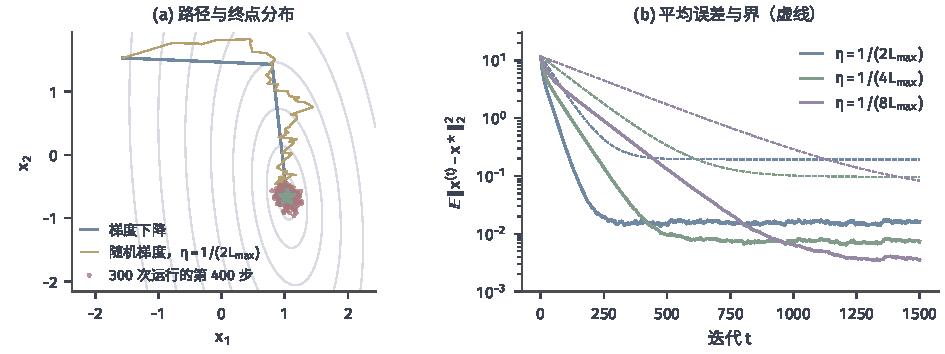
\includegraphics[width=160mm]{figures/03-optimization-evolution-and-signals/01-optimization/matplotlib/c6-sgd-noise-ball/figure.pdf}
  \caption{常数步长随机梯度下降的噪声邻域。问题是$n=40$、$d=2$的岭回归最小二乘，$\mu\approx0.304$，$L_{\max}\approx9.83$，$\sigma_\star^2\approx0.577$。(a) 灰色等高线上，蓝线为步长$1/L$的梯度下降，黄线为步长$1/(2L_{\max})$的一条随机梯度路径，红点为从最小点出发的$300$次独立运行在第$400$步的位置。(b) $400$次运行的平均平方距离（实线）与定理~\ref{thm:opt-sto-constant-step}的上界（同色虚线）。}
  \label{fig:opt-sto-noise-ball}
\end{figure*}

\paragraph{有限步结论与长期收敛}
式~\eqref{eq:opt-sto-noise-ball}是关于每个固定$t$的期望的界，不是关于单条路径的界。要让期望误差趋于零，必须让步长趋于零，下一小节给出具体的调度和速率。经典的\term{随机逼近}（stochastic approximation）理论还研究另一个问题：在$\sum_t\eta^{(t)}=\infty$、$\sum_t(\eta^{(t)})^2<\infty$等条件下，迭代点是否\emph{几乎必然}收敛\scite{math-robbins1951stochastic}。那需要鞅收敛定理来控制累积噪声，不能只靠逐步取期望得到，归第~\ref{chap:stochastic-processes-and-approximation}章。本章不把这些步长条件当作已证明的收敛保证使用。

\subsection{步长调度}
\label{sec:opt-sto-schedules}

\paragraph{几种调度规则}
定理~\ref{thm:opt-sto-constant-step}说明步长同时控制两件事：初始误差消退的速度和噪声累积的水平。按迭代推进改变步长的规则称为步长调度，在机器学习中通常叫\term{学习率调度}（learning rate scheduling）。常见的有四类。\emph{常数}步长最简单，误差停在与$\eta$成正比的平台上。\emph{预定递减}步长如$\eta^{(t)}=\eta^{(0)}/(1+t/t_0)$，事先写成迭代次数的函数。\emph{分段}步长在若干预定时刻把步长乘以一个因子，例如每$K$步减半。\emph{按观测调整}的规则读取一个监测量，例如若干步内目标估计不再下降就减小步长。

\paragraph{调度的时钟}
每种调度都依赖一个“时钟”$t$，它可以数样本读取次数、参数更新次数或数据遍历次数，三者在批量和微批量下并不相同。批量为$b$时，“每$500$步减半”与“每读取$500$个样本减半”相差$b$倍。把一个批量拆成几个微批量累积时（第~\ref{sec:opt-sto-minibatch}节），若在每个微批量之后推进时钟，步长就会比预定的更快地减小。改变时钟就改变了实际执行的算法，报告调度时必须同时说明时钟的单位。

按观测调整的规则还有一层需要检查：步长必须在抽取本步读数之前确定。若用本步读数本身决定本步步长，例如读数大时缩小步长，那么$\mathbb E_t[\eta^{(t)}\bm g^{(t)}]\neq\eta^{(t)}\nabla f(\bm x^{(t)})$，前面的单步分析就不再适用。用上一步或单独一批样本上的监测量调整则没有这个问题。

\paragraph{递减步长的速率}
在强凸情形下，适当的递减步长让期望误差以$1/t$的速度趋于零。下面的定理把这一点从同一条递推中推出。

\begin{theorem}[递减步长的期望误差]
\label{thm:opt-sto-decreasing}
在引理~\ref{lem:opt-sto-distance}的条件下设$\mu>0$，取$t_0\geq4L_{\max}/\mu$与
\[
  \eta^{(t)}=\frac{2}{\mu(t+t_0)} .
\]
则对一切$t\geq0$，$\mathbb E\lVert\bm x^{(t)}-\bm x^\star\rVert_2^2\leq\dfrac{\nu}{t+t_0}$，其中$\nu=\max\bigl\{t_0\lVert\bm x^{(0)}-\bm x^\star\rVert_2^2,\ 8\sigma_\star^2/\mu^2\bigr\}$。
\end{theorem}

\begin{proof}
由$t_0\geq4L_{\max}/\mu$，$\eta^{(t)}\leq2/(\mu t_0)\leq1/(2L_{\max})$，所以与定理~\ref{thm:opt-sto-constant-step}的证明相同，$a_t=\mathbb E\lVert\bm x^{(t)}-\bm x^\star\rVert_2^2$满足$a_{t+1}\leq(1-\mu\eta^{(t)})a_t+2(\eta^{(t)})^2\sigma_\star^2$。对$t$归纳。$t=0$时$a_0\leq\nu/t_0$由$\nu$的定义成立。设$a_t\leq\nu/k$，$k=t+t_0\geq4$，则$1-\mu\eta^{(t)}=1-2/k\geq0$，
\[
  a_{t+1}\leq\Bigl(1-\frac2k\Bigr)\frac\nu k+\frac{8\sigma_\star^2}{\mu^2k^2}
  \leq\frac{(k-2)\nu}{k^2}+\frac{\nu}{k^2}=\frac{(k-1)\nu}{k^2}\leq\frac{\nu}{k+1},
\]
其中第二步用$8\sigma_\star^2/\mu^2\leq\nu$，最后一步用$(k-1)(k+1)\leq k^2$。
\end{proof}

这条速率的代价体现在常数上：$t_0$至少是条件数$L_{\max}/\mu$的四倍，早期步长因此偏小；$\nu$中的$8\sigma_\star^2/\mu^2$说明噪声越大、曲率越小，后期误差越大。分段减半是另一种折中：在每一段用常数步长$\eta$跑到平台$2\eta\sigma_\star^2/\mu$附近，再把步长减半，平台随之减半，而下一段从更低的起点出发。图~\ref{fig:opt-sto-step-schedules}比较三种调度。常数步长最早停住；递减步长在前几百步因为步长较小而落后，此后持续下降，并始终位于定理~\ref{thm:opt-sto-decreasing}的上界之下；分段减半在每次减半后出现一个新的下降段，与递减步长在后期相当。

\begin{figure*}[!htbp]
  \centering
  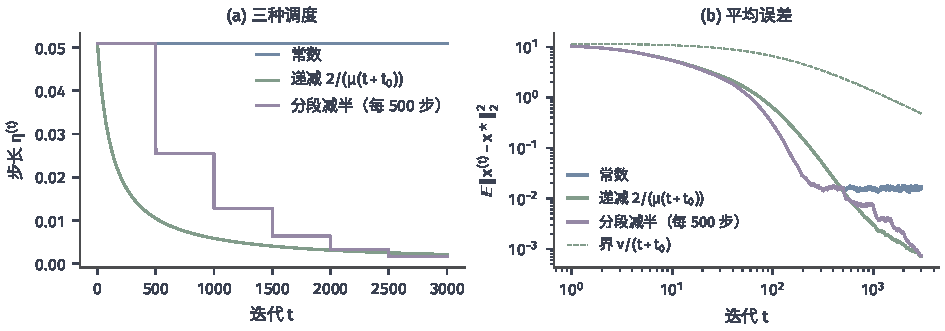
\includegraphics[width=160mm]{figures/03-optimization-evolution-and-signals/01-optimization/matplotlib/c6-step-schedules/figure.pdf}
  \caption{三种步长调度。问题同图~\ref{fig:opt-sto-noise-ball}。(a) 常数步长$\eta^{(0)}=1/(2L_{\max})\approx0.051$，递减步长$2/(\mu(t+t_0))$（$t_0=4L_{\max}/\mu\approx129$），以及每$500$步减半的分段步长。(b) $400$次运行的平均平方距离，双对数坐标；虚线是定理~\ref{thm:opt-sto-decreasing}的上界$\nu/(t+t_0)$。时钟按参数更新次数计。}
  \label{fig:opt-sto-step-schedules}
\end{figure*}

\paragraph{调度需要核验的条件}
使用任何调度，都要回到上面的递推核对三件事：每一步的步长是否满足递推成立所需的上限（这里是$\eta^{(t)}\leq1/(2L_{\max})$），步长是否在读数之前确定，以及读数是否满足所用的无偏和矩条件。步长变小时，位移变小、目标估计的波动也变小，但这只说明算法“走得慢了”，不说明已经接近最优；判断精度仍要看原目标的误差或梯度残差。另外，定理~\ref{thm:opt-sto-decreasing}给出的是期望界，一个固定的衰减公式并不自动保证每条随机路径都收敛。

\subsection{有限步误差与返回对象}
\label{sec:opt-sto-return}

前面的结论都关于“第$t$个迭代点”。实际停止时还要决定交出哪个点，而不同的返回规则配合不同的分析。本小节在凸与非凸两种情形下各给出一个有限步界，它们的返回对象并不相同。

\paragraph{凸目标与加权平均点}
不假设强凸时，到最小点的距离不再逐步收缩，但式~\eqref{eq:opt-sto-distance}中的目标差项可以被累加起来。

\begin{theorem}[凸目标的加权平均点]
\label{thm:opt-sto-convex-average}
设每个$f_i$凸且$L_{\max}$光滑，$f$有最小点$\bm x^\star$，$i^{(t)}$均匀且与历史独立，确定的步长满足$0<\eta^{(t)}\leq1/(4L_{\max})$。令$\bar{\bm x}^{(T)}=\sum_{t<T}\eta^{(t)}\bm x^{(t)}\big/\sum_{t<T}\eta^{(t)}$，则
\begin{equation}
\label{eq:opt-sto-convex-average}
  \mathbb E f(\bar{\bm x}^{(T)})-f^\star\leq\frac{\lVert\bm x^{(0)}-\bm x^\star\rVert_2^2+2\sigma_\star^2\sum_{t<T}(\eta^{(t)})^2}{\sum_{t<T}\eta^{(t)}} .
\end{equation}
\end{theorem}

\begin{proof}
在式~\eqref{eq:opt-sto-distance}中取$\mu=0$。由$\eta^{(t)}\leq1/(4L_{\max})$得$2(1-2\eta^{(t)}L_{\max})\geq1$，于是
$\eta^{(t)}\bigl(f(\bm x^{(t)})-f^\star\bigr)\leq\lVert\bm x^{(t)}-\bm x^\star\rVert_2^2-\mathbb E_t\lVert\bm x^{(t+1)}-\bm x^\star\rVert_2^2+2(\eta^{(t)})^2\sigma_\star^2$。取全期望并对$t=0,\dots,T-1$求和，距离项相消，只剩首项和一个非正的末项。最后由$f$的凸性，$f(\bar{\bm x}^{(T)})\leq\sum_t\eta^{(t)}f(\bm x^{(t)})/\sum_t\eta^{(t)}$。
\end{proof}

分子中的$\lVert\bm x^{(0)}-\bm x^\star\rVert_2^2$随总步长$\sum\eta^{(t)}$被摊薄，$2\sigma_\star^2\sum(\eta^{(t)})^2$是噪声的累积。常数步长$\eta$时右边是$\lVert\bm x^{(0)}-\bm x^\star\rVert_2^2/(\eta T)+2\eta\sigma_\star^2$，前一项要求步长大，后一项要求步长小。若预先知道总步数$T$，取$\eta=\min\{1/(4L_{\max}),\ \lVert\bm x^{(0)}-\bm x^\star\rVert_2/(\sigma_\star\sqrt{2T})\}$，代入可得
\[
  \mathbb E f(\bar{\bm x}^{(T)})-f^\star\leq\frac{4L_{\max}\lVert\bm x^{(0)}-\bm x^\star\rVert_2^2}{T}+\frac{2\sqrt2\,\sigma_\star\lVert\bm x^{(0)}-\bm x^\star\rVert_2}{\sqrt T}.
\]
无噪声时只剩$O(1/T)$，与梯度下降对凸目标的速率同阶；有噪声时$O(1/\sqrt T)$的第二项占主导。这个步长依赖于事先固定的$T$：若之后决定多跑几步，结论要按新的$T$重新核对。

\paragraph{非凸目标与随机返回点}
对非凸目标，最小点距离和目标差都不再是合适的进展度量。引理~\ref{lem:opt-sto-one-step}给出的期望下降则不依赖凸性，可以对梯度范数的平方求和。

\begin{theorem}[非凸光滑目标的随机返回点]
\label{thm:opt-sto-nonconvex}
设$f$是$L$光滑的且有下界$f_{\inf}$，读数条件无偏且$\mathbb E_t\lVert\bm g^{(t)}-\nabla f(\bm x^{(t)})\rVert_2^2\leq\sigma^2$，确定的步长满足$0<\eta^{(t)}\leq1/L$。运行结束后与算法独立地抽取$\tau\in\{0,\dots,T-1\}$，$\mathbb P(\tau=t)=\eta^{(t)}/\sum_{s<T}\eta^{(s)}$，返回$\bm x^{(\tau)}$。则
\begin{equation}
\label{eq:opt-sto-nonconvex}
  \mathbb E\lVert\nabla f(\bm x^{(\tau)})\rVert_2^2\leq\frac{2\bigl(f(\bm x^{(0)})-f_{\inf}\bigr)+L\sigma^2\sum_{t<T}(\eta^{(t)})^2}{\sum_{t<T}\eta^{(t)}} .
\end{equation}
\end{theorem}

\begin{proof}
$\eta^{(t)}\leq1/L$使式~\eqref{eq:opt-sto-one-step}中$1-L\eta^{(t)}/2\geq1/2$，于是$\tfrac{\eta^{(t)}}2\lVert\nabla f(\bm x^{(t)})\rVert_2^2\leq f(\bm x^{(t)})-\mathbb E_tf(\bm x^{(t+1)})+\tfrac L2(\eta^{(t)})^2\sigma^2$。取全期望，对$t<T$求和，目标值项相消，剩下$f(\bm x^{(0)})-\mathbb Ef(\bm x^{(T)})\leq f(\bm x^{(0)})-f_{\inf}$。由$\tau$的分布，$\mathbb E\lVert\nabla f(\bm x^{(\tau)})\rVert_2^2=\sum_t\eta^{(t)}\mathbb E\lVert\nabla f(\bm x^{(t)})\rVert_2^2/\sum_t\eta^{(t)}$，代入即得。
\end{proof}

常数步长时，右边是$2(f(\bm x^{(0)})-f_{\inf})/(\eta T)+L\eta\sigma^2$，与凸情形结构相同；取$\eta=\min\{1/L,\sqrt{2(f(\bm x^{(0)})-f_{\inf})/(L\sigma^2T)}\}$得到$O(1/T+1/\sqrt T)$的梯度平方残差\scite{ghadimi2013stochastic}。随机返回点是证明的需要：这个界控制的是梯度平方的加权平均，而不是最后一点。实践中常改为返回在独立样本上估计梯度范数最小的迭代点，那是另一个返回规则，需要另算估计误差。

\paragraph{三种返回对象}
最后一点、加权平均点和随机返回点是三个不同的随机向量，上面的定理分别只对其中一个成立。凸情形的界针对平均点；最后一点在强凸、常数步长时满足定理~\ref{thm:opt-sto-constant-step}，误差停在噪声平台上。图~\ref{fig:opt-sto-return-points}在二维最小二乘上比较它们：单次运行的最后一点剧烈波动，最后一点的平均误差停在约$8.6\times10^{-3}$；从头开始的平均点受早期远离最小点的迭代拖累，下降较慢，却没有平台；只平均后半程迭代的点兼顾两者，在$4000$步时约为$1.4\times10^{-4}$。平均能越过平台，是因为在二次目标上读数关于$\bm x$是线性的，期望迭代满足$\mathbb E\bm x^{(t+1)}-\bm x^\star=(\bm I-\eta\nabla^2f)(\mathbb E\bm x^{(t)}-\bm x^\star)$，噪声只造成围绕最小点的对称波动；这种\term{迭代平均}（iterate averaging）对二次目标与一般强凸光滑目标的渐近效果另有专门的分析\scite{polyak1992acceleration}，非二次目标上常数步长的平均点一般带有$O(\eta)$的偏差，不能把图中的结果当作普遍结论。

\begin{figure}[!htbp]
  \centering
  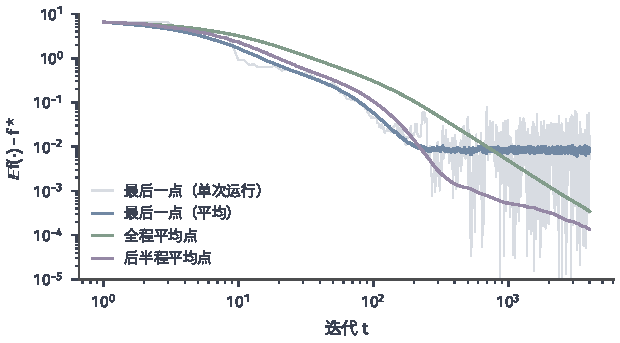
\includegraphics[width=105mm]{figures/03-optimization-evolution-and-signals/01-optimization/matplotlib/c6-return-points/figure.pdf}
  \caption{同一组运行的三种返回对象。问题同图~\ref{fig:opt-sto-noise-ball}，常数步长$1/(2L_{\max})$，$300$次运行。浅灰线为单次运行最后一点的目标差；蓝、绿、紫线分别是最后一点、全程平均点$\frac1{t+1}\sum_{s\leq t}\bm x^{(s)}$和后半程平均点$\frac{1}{t-\lfloor t/2\rfloor+1}\sum_{s=\lfloor t/2\rfloor}^{t}\bm x^{(s)}$的平均目标差，双对数坐标。}
  \label{fig:opt-sto-return-points}
\end{figure}

\paragraph{期望界的含义}
本节的结论都是期望界。若$\mathbb E[f(\bar{\bm x}^{(T)})-f^\star]\leq\varepsilon$，由Markov不等式，$\mathbb P\bigl(f(\bar{\bm x}^{(T)})-f^\star\geq\varepsilon/\delta\bigr)\leq\delta$，即以至少$1-\delta$的概率误差不超过$\varepsilon/\delta$；更紧的高概率界需要读数尾部的额外假设。期望趋于零也只蕴含依概率收敛，不蕴含几乎必然收敛，各种收敛方式之间的关系见\BookChapterRef{chap:random-variable-convergence}{卷二“随机变量的收敛与积分极限”章}。完整的鞅收敛论证、随机逼近的常微分方程解释以及长期极限都在第~\ref{chap:stochastic-processes-and-approximation}章接续，它们不是本章算法定义的前置知识。
